%------------------------------------------------------------------------------
\chapter{Hohlraumresonatoren}
\label{sec:hohlraumresonatoren}
%------------------------------------------------------------------------------


%------------------------------------------------------------------------------
\section{Elektromagnetische Felder in Hohlraumresonatoren}
%------------------------------------------------------------------------------
Ein Hohlraumresonator besteht aus einem evakuierten Hohlraum, welcher durch ein leitendes Material begrenzt wird.
Die im Hohlraum propagierenden elektromagnetischen Wellen werden an den leitenden Wänden reflektiert und führen zur Ausbildung von stehenden elektromagnetischen Wellen im Resonatorinnenraum, welche unter anderem zur Beschleunigung von elektrisch geladenen Teilchen genutzt werden können.
Aufgrund der Randbedingungen an der näherungsweise ideal leitenden Grenzfläche müssen die folgenden Anforderungen an das elektromagnetische Feld gestellt werden:
\begin{align}
  E_\parallel = 0 \qquad \text{und} \qquad B_\perp = 0\text{,}
  \label{eq:randbedingung_leiter}
\end{align}
wobei $E_\parallel$ die Tangentialkomponente und $B_\perp$ die Normalkomponente des elektrischen bzw.\ magnetischen Feldes auf der Grenzfläche kennzeichnet.
Die Lösung der \textsc{Maxwell}-Gleichungen unter Beachtung dieser Grenzbedingungen zeigt, dass in Abhängigkeit der Geometrie des Hohlraums, eine unbegrenzte Anzahl von Moden mit bestimmten Frequenzen im Resonator auftreten können.
Die Klassifizierung der einzelnen Moden erfolgt dabei anhand ihrer Feldkonfiguration relativ zur Propagationsrichtung der hin- und rücklaufenden Wellen im Resonator.
Dabei unterscheidet man zwischen transversal-elektrischen (TE)-Moden, welche lediglich transversale elektrische und longitudinal magnetische Felder aufweisen und transversal-magnetischen (TM)-Moden, bei denen der umgekehrte Fall eintritt.

Viele der in Beschleunigern verwendeten Kavitäten\footnote{von lat.\ \emph{cavum} "Höhle": Hohlraumresonator oftmals engl. \emph{Cavity}} basieren auf kreiszylindrischen Resonatoren\footnote{engl. \emph{Pillbox-Cavities}, für deren Ähnlichkeit mit einer Tablettenschachtel}, welche eine analytische Lösung der \textsc{Maxwell}-Gleichungen erlauben.
Daher soll im Folgenden die Feldkonfiguration der verschiedenen Moden in einem solchen Resonator dargestellt werden und die in dieser Arbeit verwendete Notation eingeführt werden.
Dabei genügt die Betrachtung der longitudinalen Felder eines zylindrischen Hohlraums mit Radius~$R$ und Länge~$L$ in Zylinderkoordinaten $(r, \theta, z)$, da durch diese die transversalen Feldkomponenten eindeutig festgelegt sind \cite[S.\ 4]{hillert}.
Man findet für die Moden in dem kreiszylindrischen Resonator \cite[S. 28-32]{wangler}:
\begin{subequations}
  \begin{align}
  \mathrm{TM}_{mnp}\text{-Mode:} \quad E_z = E_0 J_m(k_{mn} r) \cos(m \theta) \cos\left(\frac{p \pi z}{L}\right) \exp(i \omega_{mnp} t) \qquad B_z = 0\\
  \mathrm{TE}_{mnp}\text{-Mode:} \quad B_z = B_0 J_m(k_{mn}^\prime r) \cos(m \theta) \sin\left(\frac{p \pi z}{L}\right) \exp(i \omega_{mnp}^\prime t) \qquad  E_z = 0
  \end{align}
  \label{eqs:felder_pillbox}
\end{subequations}
wobei die Konstante $k_{mn}^{(\prime)}$ definiert ist als:
\begin{align}
k_{mn}^{(\prime)} := \frac{x_{mn}^{(\prime)}}{R}
\end{align}
mit der $n$-ten positiven Nullstelle $x_{mn}$ Besselfunktion $m$-ter Ordnung $J_m(x)$ respektive ihrer Ableitung $J_m^\prime(x)$.
Aus den Gleichungen \eqref{eqs:felder_pillbox} folgt dann die Bedeutung der Indizes $m, n$ und $p$:
Der Index $m$ ($m=0, 1, \dots$) beschreibt die Periodenzahl der Feldkomponente in azimutaler Richtung.
Weiterhin wird durch $n$ ($n=1, 2, \dots$) die Anzahl der Knoten der longitudinalen Feldkomponente in radialer Richtung (ausgenommen Knoten im Ursprung mit $r=0$) gegeben.
Schließlich gibt der Index $p$ (TM-Mode: $p= 0, 1, \dots$; TE-Mode: $p = 1, 2, \dots$) die Anzahl der halben Perioden in longitudinaler Richtung an.
Die Kreisfrequenz~$\omega_{mnp}$ der einzelnen Moden ist dabei gegeben durch \cite[S.28-32]{wangler}:
\begin{align}
\omega_{mnp}^{(\prime)} = c \cdot \sqrt{\left( k_{mn}^{(\prime)}\right)^2 + \left( \frac{p \pi}{L} \right)^2}
\end{align}

Eine analytische Berechnung der Moden von komplexeren Resonatorgeometrien ist im Allgemeinen nicht möglich und es muss auf numerische Methoden zurückgegriffen werden.
Dazu wird in dieser Arbeit \emph{CST Microwave Studio\textsuperscript{\textregistered}} verwendet, welches die Lösung der Maxwell-Gleichungen diskretisiert und auf ein Eigenwertproblem zurückführt.


%------------------------------------------------------------------------------
\section{Kenngrößen von Resonatoren am Modell des RLC-Parallelkreises}
%------------------------------------------------------------------------------
\begin{figure}[h]
  \centering
  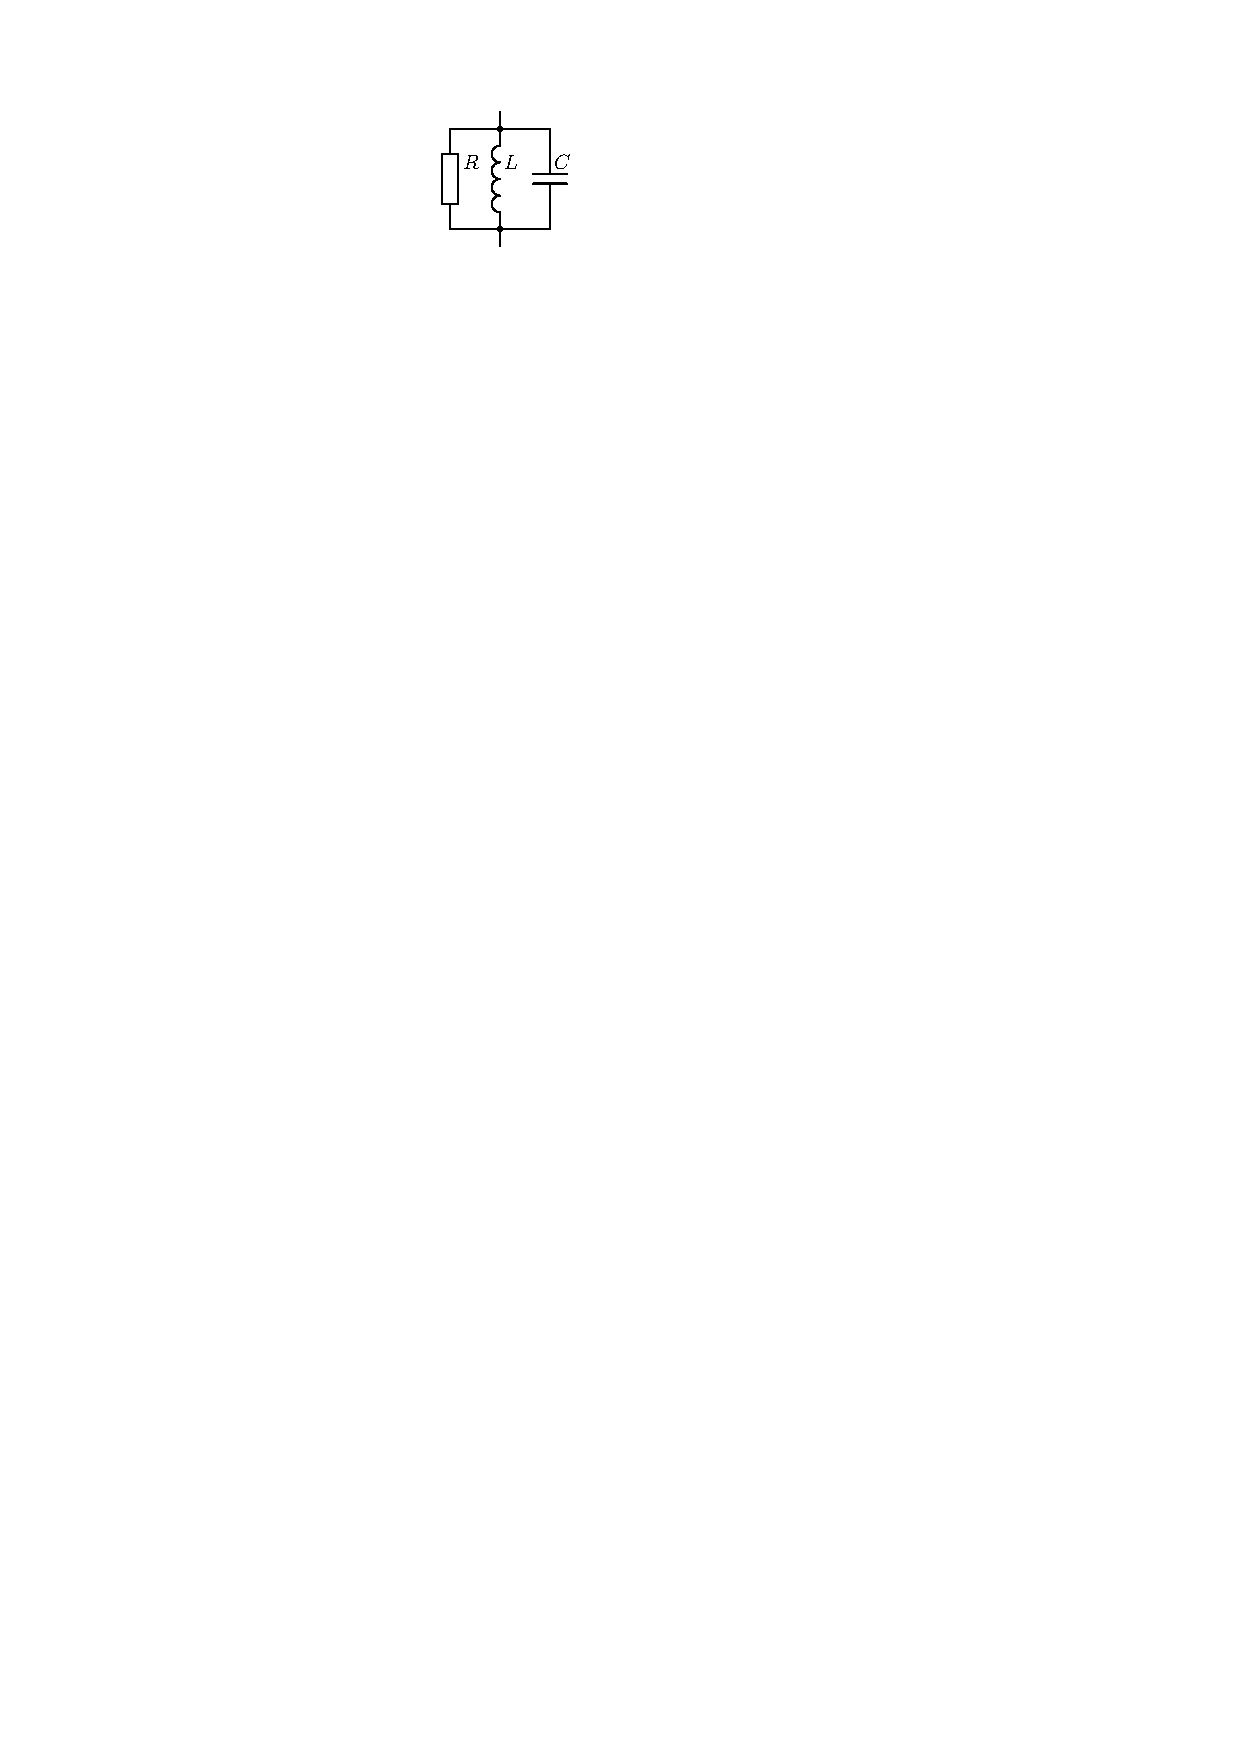
\includegraphics[scale=1.4]{./figs/RLC_circuit.pdf}
  \caption{Ein getriebener Parallelschwingkreis bestehend aus dem ohm'schen Widerstand~$R$, der Induktivität~$L$ und der Kapazität~$C$ als Modell für die elektrischen Eigenschaften eines Hohlraumresonators in der Nähe einer Resonanz.}
  \label{fig:rlc_circuit}
\end{figure}
Die elektrischen Eigenschaften von Hohlraumresonatoren können in einem kleinen Frequenzbereich um eine Resonanz durch das Modell des Parallelschwingkreises (siehe Abb.\ \ref{fig:rlc_circuit}) erklärt werden.
Zur vollständigen Beschreibung ist die Angabe der drei Kenngrößen: Widerstand~$R$, Induktivität~$L$ und Kapazität~$C$ ausreichend.
Für die Behandlung von Hohlraumresonatoren ist es zweckmäßig andere Parameter zur Beschreibung zu wählen.
Daher verwendet man stattdessen die Eigenfrequenz~$\omega_0$, die Kreisgüte~$Q_0$ und der Widerstand~$R$ des Schwingkreises zur Beschreibung.
Die Eigenfrequenz des Kreises folgt aus der \textsc{Thomson}schen Schwingungsgleichung:
\begin{align}
  \omega_0 = \frac{1}{\sqrt{L C}}
\end{align}
und die Kreisgüte aus ihrer Definition:
\begin{align}
  Q_0 &\coloneqq 2\pi \cdot \frac{\text{gespeicherte Energie}}{\text{Energieverlust pro Periode}} = \frac{\omega_0 W_0}{P_\mathrm{V}} = \omega_0 R C
  \label{eq:def_guete}
\end{align}
mit der im Kreis gespeicherten Energie $W_0$ und der Verlustleistung $P_\mathrm{V}$ aufgrund des ohm'schen Widerstandes $R$.
Nach der Einführung dieser Kenngrößen kann die Impedanz des Kreises beziehungsweise des Hohlraumresonators ausgedrückt werden als:
\begin{align}
  Z(\omega) = \frac{R}{1 + i Q_0 \left( \frac{\omega}{\omega_0}  - \frac{\omega_0}{\omega}\right)}
\end{align}

\begin{figure}[h]
  \centering
  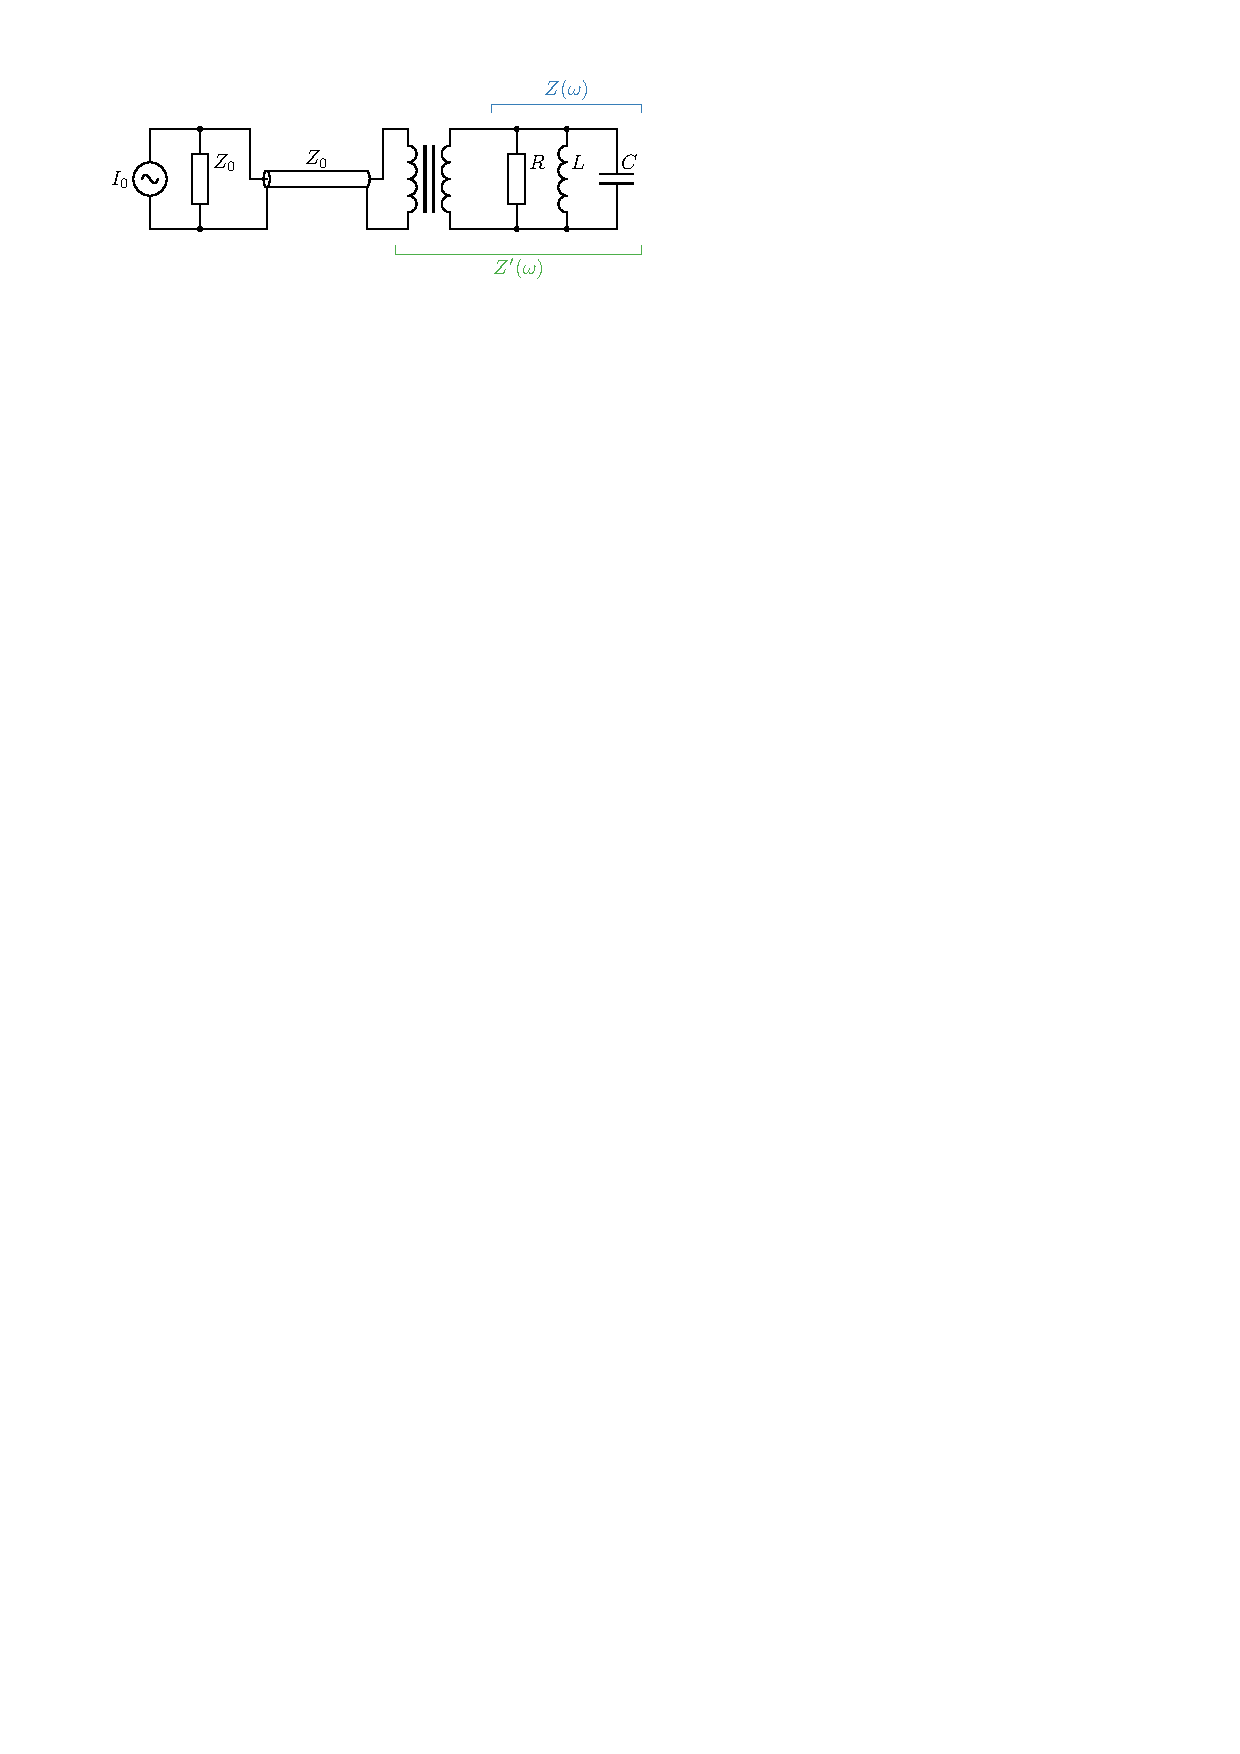
\includegraphics[scale=1.4]{./figs/RLC_coupling.pdf}
  \caption{Modell der induktiven Kopplung eines treibenden Hochfrequenzsignals $U_0$ über die Koppelschleife an den Resonator. Die Signalquelle ist mit einem Wellenleiter charakteristischer Impedanz~$Z_0$ mit der Koppelschleife verbunden. \todo{$Z$ und $Z^\prime$}}
  \label{fig:rlc_coupling}
\end{figure}
Bisher war die Betrachtung auf ungetriebene Resonatoren beschränkt und soll nun auf die Anregung durch ein externes Hochfrequenzsignal erweitert werden.
Zur Übertragung der Leistung aus einem Wellenleiter mit charakteristischer Impedanz $Z_0$ in eine Schwingungsmode der Kavität können verschiedene Methoden verwendet werden.
Eine ist die induktive Kopplung an das Magnetfeld der Mode, bei der der Wellenleiter mit einer Leiterschleife (die sog.\ Koppelschleife) im Resonator verbunden ist.
Dadurch wird in der Leiterschleife ein hochfrequenter Wechselstrom angeregt, welcher ein zeitlich veränderliches Magnetfeld erzeugt. Dieses kann an das Magnetfeld verschiedener Moden der Kavität koppeln und diese resonant anregen\footnote{Dies ist nur möglich wenn die jeweilige Mode am Ort der Koppelschleife ein nicht verschwindendes Magnetfeld besitzt.}.

Im Modell des Parallelschwingkreises bedeutet dies, dass die Impedanz~$Z(\omega)$ der Kavität durch die induktive Kopplung transformiert wird.
Direkt hinter der Koppelschleife habe der Resonator die transformierte Impedanz $Z^\prime(\omega)$.
Man definiert als Maß für die Kopplung den sog.\ Koppelfaktor:
\begin{align}
  \kappa \coloneqq \frac{Z^\prime(\omega_0)}{Z_0}
  \label{eq:koppelfaktor}
\end{align}
mit dem Wellenwiderstand~$Z_0$ des Wellenleiters und unterscheidet zwischen unterkritischer $(\kappa < 1)$, kritischer $(\kappa = 1)$ und überkritischer Kopplung $(\kappa > 1)$.
Im Falle von resonanter Anregung bei kritischer Kopplung folgert man aus Gleichung \eqref{eq:koppelfaktor}, dass der Wellenleiter mit seiner charakteristischen Impedanz abgeschlossen ist und somit keine Reflexionen an der Koppelschleife entstehen.
Mit der Definition des Koppelfaktors und der Proportionalität $Z^\prime(\omega) \propto Z(\omega)$ für ideale Transformatoren folgt die Frequenzabhängigkeit der Impedanz $Z^\prime(\omega)$ des Systems bestehend aus Koppelschleife und Resonator:
\begin{align}
  Z^\prime(\omega) = \kappa \frac{Z_0}{R} Z(\omega)
  \label{eq:impedanz_hinter_schleife}
\end{align}

Von besonderem Interesse ist der komplexe Reflexionskoeffizient $\rho$ zwischen Wellenleiter und Koppelschleife, da dieser direkt mit einem vektoriellen Netzwerkanalysators\footnote{kurz: VNA} zu messen ist.
Er beschreibt das Verhältnis der komplexen Spannungsamplituden von hin- und rücklaufender Welle in einem Wellenleiter.
Aus der Leitungstheorie \cite[S.\ 57]{pozar} folgt für den Reflexionskoeffizienten am Übergang von einem Wellenleiter mit Wellenwiderstand $Z_0$ auf eine Abschlussimpedanz~$Z^\prime$:
\begin{align}
  \rho = \frac{Z^\prime - Z_0}{Z^\prime + Z_0}
  \label{eq:reflexionskoeff_trans_line}
\end{align}
Es folgt nach Einsetzen von \eqref{eq:impedanz_hinter_schleife} in \eqref{eq:reflexionskoeff_trans_line} der Ausdruck für den Reflexionskoeffizienten 
\begin{align}
  \rho(\omega) = \frac{\frac{\kappa}{R} \cdot Z(\omega) - 1}{\frac{\kappa}{R} \cdot Z(\omega) + 1} = \frac{(\kappa - 1) + i  Q_0 \left( \frac{\omega}{\omega_0}  - \frac{\omega_0}{\omega}\right)}{\left( \kappa + 1 \right) + i  Q_0 \left( \frac{\omega}{\omega_0}  - \frac{\omega_0}{\omega}\right)}
\end{align}
\todo{Abschlusssatz}


%------------------------------------------------------------------------------
\section{Kopplung mehrerer Resonatoren}
%------------------------------------------------------------------------------


%------------------------------------------------------------------------------
\section{Resonante Störkörpermessung}
%------------------------------------------------------------------------------
\todo{Vernachlässigung von Luft $\mu$, $\epsilon$}
Die resonante\footnote{\todo{Was ist nicht resonante SKM?}} Störkörpermessung basiert auf der Störung eines Hohlraumresonators durch einen dielektrischen oder magnetischen Körper (dem sog.\ Störkörper), welcher durch das Feld im Resonator polarisiert beziehungsweise magnetisiert wird.
Eine solche lokalisierte Störung verursacht eine Verschiebung der Resonanzfrequenz~$\Delta \omega$ in Abhängigkeit des elektrischen und magnetischen Feldes am Ort des Störkörpers.
Quantitativ kann die Verschiebung beschrieben werden durch (für eine Herleitung siehe Anhang \ref{app:herleitung_frequenzverschiebung}):
\begin{align}
  \frac{\Delta \omega}{\omega_0} = - \frac{\int_V \mathrm{d}V \left[ \ve_0^* \cdot \vec{P} + \vb_0^* \cdot \vec{M} \right]}{4 W_0}
  \label{eq:frequenzverschiebung}
\end{align}
mit dem Resonatorvolumen~$V$, der Polarisation~$\vec{P}$, der Magnetisierung~$\vec{M}$, der im elektromagnetischen Feld gespeicherten Energie~$W_0$ und den komplex konjugierten Feldern $\ve_0^*, \vb_0^*$ des ungestörten Resonators.

Im Rahmen dieser Arbeit wird eine dielektrische Kugel mit relativer elektrischer Permittivität~$\epsilon_\mathrm{r}$ verwendet.
Darüber hinaus sei die magnetische Permeablität~$\mu$ vernachlässigbar, sodass es zu keiner Magnetisierung ($\vec{M} = 0$) des Störkörpers kommt.
Weiterhin wird angenommen, dass das Volumen des kugelförmigen Störkörpers wesentlich kleiner ist als das Resonatorvolumen, sodass am Ort des Störkörpers das elektrische Feld als homogen angesehen werden kann.
Dadurch kann die Polarisation $\vec{P}$ der dielektrischen Kugel im homogenen elektrischen Feld $\ve_0$ ausgedrückt werden als \cite{jackson} (S.115):
\begin{align}
  \vec{P} = 3 \, \frac{\epsilon_\mathrm{r} - 1}{\epsilon_\mathrm{r} + 2} \, \epsilon_0 \ve_0
  \label{eq:polarisation_kugel}
\end{align}
mit der elektrischen Feldkonstante~$\epsilon_0$.
Durch die Annahme der Homogenität der Felder und verschwindender Polarisation und Magnetisierung außerhalb des Störkörpervolumens~$V_\mathrm{s}$ kann direkt crcdie Amplitude $|\ve_0|$ des elektrischen Feldes am Ort des Störkörpers berechnet werden:\todo{Übergang unklar, vorallem was Positionsabhängigkeit der Felder angeht und Verschwindender Polarisation/Magnetisierung im Resonatorvolumen, negatives Vorzeichen in der Wurzel}
\begin{align}
  |\ve_0| = \sqrt{-4 \cdot \frac{W_0}{\alpha_\mathrm{s}} \cdot \frac{\Delta \omega}{\omega_0}} \label{eq:skm_e_feld}
\end{align}
wobei man die sogenannte Störkörperkonstante $\alpha_\mathrm{s}$ definiert:
\begin{align}
  \alpha_\mathrm{s} \coloneqq 3 \, \frac{\epsilon_\mathrm{r} - 1}{\epsilon_\mathrm{r} + 2} \, \epsilon_0 V_\mathrm{s}
\end{align}
Die Amplitude des elektrischen Feldes in Gleichung \eqref{eq:skm_e_feld} ist von der im Resonator gespeicherten Energie $W_0$ abhängig, welche wiederum von der in den Resonator eingekoppelten Leistung abhängt.
Daher ist es zweckmäßig die gespeicherte Energie $W_0$ über Gleichung \eqref{eq:def_guete} in abhängigkeit der Güte $Q_0$ und Verlustleistung $P_\mathrm{V}$ auszudrücken.
Die Amplitude des elektrischen Feldes kann dann auf die Wurzel der Verlustleistung normiert werden und man erhält:
\begin{align}
  \frac{|\ve_0|}{\sqrt{P_\mathrm{V}}} = \sqrt{-4 \cdot \frac{Q_0}{\alpha_s} \cdot \frac{\Delta \omega}{\omega_0^2}}
\end{align}


%------------------------------------------------------------------------------
\section{Makroskopische Kenngrößen}
%------------------------------------------------------------------------------
